\documentclass[1p]{elsarticle_modified}
%\bibliographystyle{elsarticle-num}

%\usepackage[colorlinks]{hyperref}
%\usepackage{abbrmath_seonhwa} %\Abb, \Ascr, \Acal ,\Abf, \Afrak
\usepackage{amsfonts}
\usepackage{amssymb}
\usepackage{amsmath}
\usepackage{amsthm}
\usepackage{scalefnt}
\usepackage{amsbsy}
\usepackage{kotex}
\usepackage{caption}
\usepackage{subfig}
\usepackage{color}
\usepackage{graphicx}
\usepackage{xcolor} %% white, black, red, green, blue, cyan, magenta, yellow
\usepackage{float}
\usepackage{setspace}
\usepackage{hyperref}

\usepackage{tikz}
\usetikzlibrary{arrows}

\usepackage{multirow}
\usepackage{array} % fixed length table
\usepackage{hhline}

%%%%%%%%%%%%%%%%%%%%%
\makeatletter
\renewcommand*\env@matrix[1][\arraystretch]{%
	\edef\arraystretch{#1}%
	\hskip -\arraycolsep
	\let\@ifnextchar\new@ifnextchar
	\array{*\c@MaxMatrixCols c}}
\makeatother %https://tex.stackexchange.com/questions/14071/how-can-i-increase-the-line-spacing-in-a-matrix
%%%%%%%%%%%%%%%

\usepackage[normalem]{ulem}

\newcommand{\msout}[1]{\ifmmode\text{\sout{\ensuremath{#1}}}\else\sout{#1}\fi}
%SOURCE: \msout is \stkout macro in https://tex.stackexchange.com/questions/20609/strikeout-in-math-mode

\newcommand{\cancel}[1]{
	\ifmmode
	{\color{red}\msout{#1}}
	\else
	{\color{red}\sout{#1}}
	\fi
}

\newcommand{\add}[1]{
	{\color{blue}\uwave{#1}}
}

\newcommand{\replace}[2]{
	\ifmmode
	{\color{red}\msout{#1}}{\color{blue}\uwave{#2}}
	\else
	{\color{red}\sout{#1}}{\color{blue}\uwave{#2}}
	\fi
}

\newcommand{\Sol}{\mathcal{S}} %segment
\newcommand{\D}{D} %diagram
\newcommand{\A}{\mathcal{A}} %arc


%%%%%%%%%%%%%%%%%%%%%%%%%%%%%5 test

\def\sl{\operatorname{\textup{SL}}(2,\Cbb)}
\def\psl{\operatorname{\textup{PSL}}(2,\Cbb)}
\def\quan{\mkern 1mu \triangleright \mkern 1mu}

\theoremstyle{definition}
\newtheorem{thm}{Theorem}[section]
\newtheorem{prop}[thm]{Proposition}
\newtheorem{lem}[thm]{Lemma}
\newtheorem{ques}[thm]{Question}
\newtheorem{cor}[thm]{Corollary}
\newtheorem{defn}[thm]{Definition}
\newtheorem{exam}[thm]{Example}
\newtheorem{rmk}[thm]{Remark}
\newtheorem{alg}[thm]{Algorithm}

\newcommand{\I}{\sqrt{-1}}
\begin{document}

%\begin{frontmatter}
%
%\title{Boundary parabolic representations of knots up to 8 crossings}
%
%%% Group authors per affiliation:
%\author{Yunhi Cho} 
%\address{Department of Mathematics, University of Seoul, Seoul, Korea}
%\ead{yhcho@uos.ac.kr}
%
%
%\author{Seonhwa Kim} %\fnref{s_kim}}
%\address{Center for Geometry and Physics, Institute for Basic Science, Pohang, 37673, Korea}
%\ead{ryeona17@ibs.re.kr}
%
%\author{Hyuk Kim}
%\address{Department of Mathematical Sciences, Seoul National University, Seoul 08826, Korea}
%\ead{hyukkim@snu.ac.kr}
%
%\author{Seokbeom Yoon}
%\address{Department of Mathematical Sciences, Seoul National University, Seoul, 08826,  Korea}
%\ead{sbyoon15@snu.ac.kr}
%
%\begin{abstract}
%We find all boundary parabolic representation of knots up to 8 crossings.
%
%\end{abstract}
%\begin{keyword}
%    \MSC[2010] 57M25 
%\end{keyword}
%
%\end{frontmatter}

%\linenumbers
%\tableofcontents
%
\newcommand\colored[1]{\textcolor{white}{\rule[-0.35ex]{0.8em}{1.4ex}}\kern-0.8em\color{red} #1}%
%\newcommand\colored[1]{\textcolor{white}{ #1}\kern-2.17ex	\textcolor{white}{ #1}\kern-1.81ex	\textcolor{white}{ #1}\kern-2.15ex\color{red}#1	}

{\Large $\underline{10_{57}~(K10a_{6})}$}

\setlength{\tabcolsep}{10pt}
\renewcommand{\arraystretch}{1.6}
\vspace{1cm}\begin{tabular}{m{100pt}>{\centering\arraybackslash}m{274pt}}
\multirow{5}{120pt}{
	\centering
	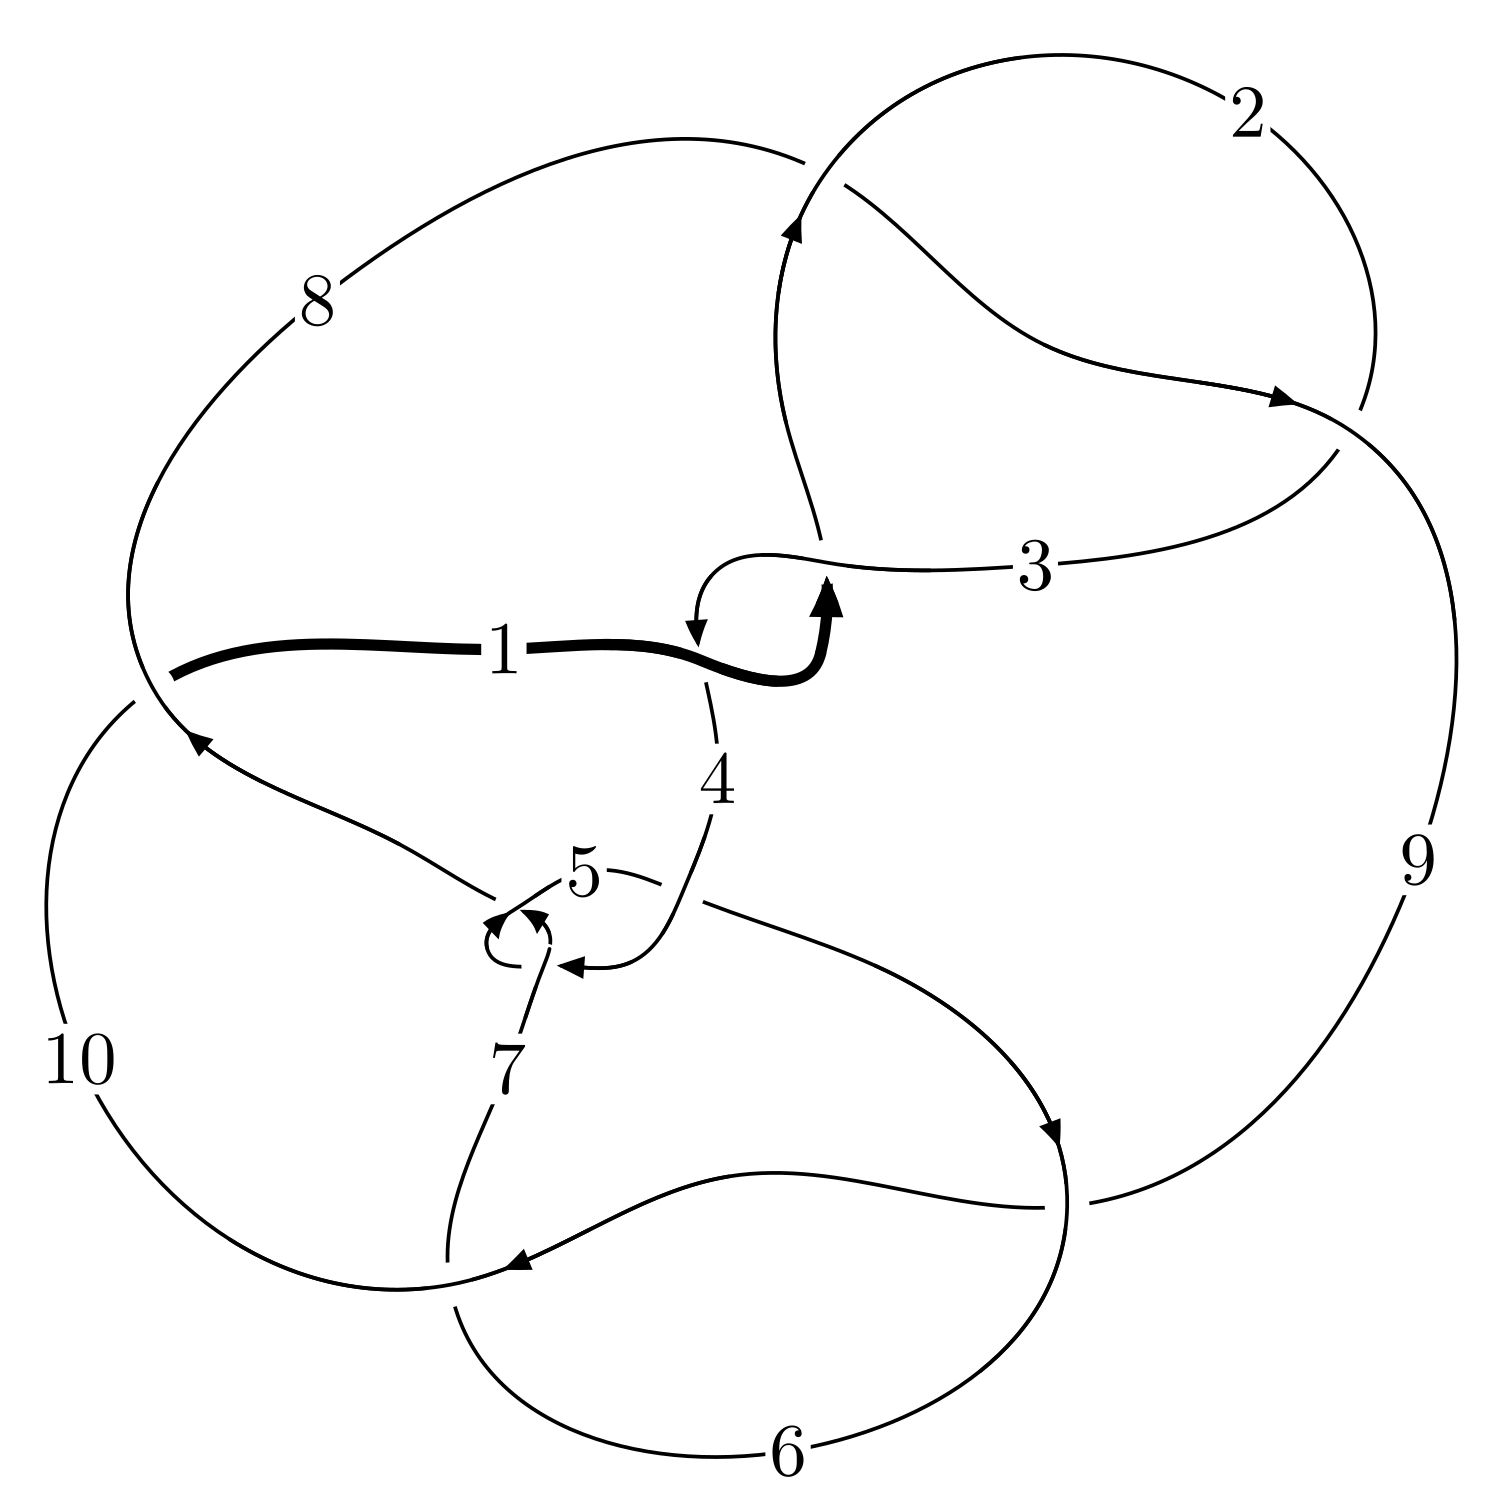
\includegraphics[width=112pt]{../../../GIT/diagram.site/Diagrams/png/141_10_57.png}\\
\ \ \ A knot diagram\footnotemark}&
\allowdisplaybreaks
\textbf{Linearized knot diagam} \\
\cline{2-2}
 &
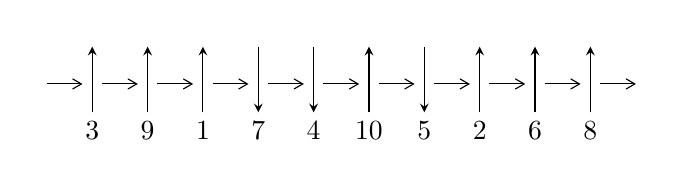
\begin{tikzpicture}[x=20pt, y=17pt]
	% nodes
	\node (C0) at (0, 0) {};
	\node (C1) at (1, 0) {};
	\node (C1U) at (1, +1) {};
	\node (C1D) at (1, -1) {3};

	\node (C2) at (2, 0) {};
	\node (C2U) at (2, +1) {};
	\node (C2D) at (2, -1) {9};

	\node (C3) at (3, 0) {};
	\node (C3U) at (3, +1) {};
	\node (C3D) at (3, -1) {1};

	\node (C4) at (4, 0) {};
	\node (C4U) at (4, +1) {};
	\node (C4D) at (4, -1) {7};

	\node (C5) at (5, 0) {};
	\node (C5U) at (5, +1) {};
	\node (C5D) at (5, -1) {4};

	\node (C6) at (6, 0) {};
	\node (C6U) at (6, +1) {};
	\node (C6D) at (6, -1) {10};

	\node (C7) at (7, 0) {};
	\node (C7U) at (7, +1) {};
	\node (C7D) at (7, -1) {5};

	\node (C8) at (8, 0) {};
	\node (C8U) at (8, +1) {};
	\node (C8D) at (8, -1) {2};

	\node (C9) at (9, 0) {};
	\node (C9U) at (9, +1) {};
	\node (C9D) at (9, -1) {6};

	\node (C10) at (10, 0) {};
	\node (C10U) at (10, +1) {};
	\node (C10D) at (10, -1) {8};
	\node (C11) at (11, 0) {};

	% arrows
	\draw[->,>={angle 60}]
	(C0) edge (C1) (C1) edge (C2) (C2) edge (C3) (C3) edge (C4) (C4) edge (C5) (C5) edge (C6) (C6) edge (C7) (C7) edge (C8) (C8) edge (C9) (C9) edge (C10) (C10) edge (C11) ;	\draw[->,>=stealth]
	(C1D) edge (C1U) (C2D) edge (C2U) (C3D) edge (C3U) (C4U) edge (C4D) (C5U) edge (C5D) (C6D) edge (C6U) (C7U) edge (C7D) (C8D) edge (C8U) (C9D) edge (C9U) (C10D) edge (C10U) ;
	\end{tikzpicture} \\
\hhline{~~} \\& 
\textbf{Solving Sequence} \\ \cline{2-2} 
 &
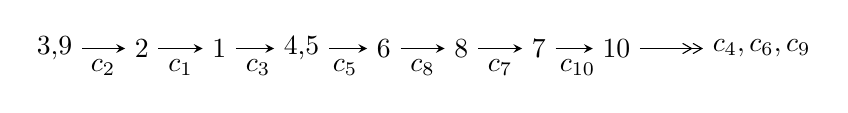
\begin{tikzpicture}[x=28pt, y=7pt]
	% node
	\node (A0) at (-1/8, 0) {3,9};
	\node (A1) at (1, 0) {2};
	\node (A2) at (2, 0) {1};
	\node (A3) at (49/16, 0) {4,5};
	\node (A4) at (33/8, 0) {6};
	\node (A5) at (41/8, 0) {8};
	\node (A6) at (49/8, 0) {7};
	\node (A7) at (57/8, 0) {10};
	\node (C1) at (1/2, -1) {$c_{2}$};
	\node (C2) at (3/2, -1) {$c_{1}$};
	\node (C3) at (5/2, -1) {$c_{3}$};
	\node (C4) at (29/8, -1) {$c_{5}$};
	\node (C5) at (37/8, -1) {$c_{8}$};
	\node (C6) at (45/8, -1) {$c_{7}$};
	\node (C7) at (53/8, -1) {$c_{10}$};
	\node (A8) at (9, 0) {$c_{4},c_{6},c_{9}$};

	% edge
	\draw[->,>=stealth]	
	(A0) edge (A1) (A1) edge (A2) (A2) edge (A3) (A3) edge (A4) (A4) edge (A5) (A5) edge (A6) (A6) edge (A7) ;
	\draw[->>,>={angle 60}]	
	(A7) edge (A8);
\end{tikzpicture} \\ 

\end{tabular} \\

\footnotetext{
The image of knot diagram is generated by the software ``\textbf{Draw programme}" developed by Andrew Bartholomew(\url{http://www.layer8.co.uk/maths/draw/index.htm\#Running-draw}), where we modified some parts for our purpose(\url{https://github.com/CATsTAILs/LinksPainter}).
}\phantom \\ \newline 
\centering \textbf{Ideals for irreducible components\footnotemark of $X_{\text{par}}$} 
 
\begin{align*}
I^u_{1}&=\langle 
- u^{40}+u^{39}+\cdots+2 u^2+b,\;u^{25}-4 u^{23}+\cdots+a-3 u,\;u^{42}-2 u^{41}+\cdots+2 u-1\rangle \\
I^u_{2}&=\langle 
b-1,\;a- u,\;u^3+u^2-1\rangle \\
\\
\end{align*}
\raggedright * 2 irreducible components of $\dim_{\mathbb{C}}=0$, with total 45 representations.\\
\footnotetext{All coefficients of polynomials are rational numbers. But the coefficients are sometimes approximated in decimal forms when there is not enough margin.}
\newpage
\renewcommand{\arraystretch}{1}
\centering \section*{I. $I^u_{1}= \langle - u^{40}+u^{39}+\cdots+2 u^2+b,\;u^{25}-4 u^{23}+\cdots+a-3 u,\;u^{42}-2 u^{41}+\cdots+2 u-1 \rangle$}
\flushleft \textbf{(i) Arc colorings}\\
\begin{tabular}{m{7pt} m{180pt} m{7pt} m{180pt} }
\flushright $a_{3}=$&$\begin{pmatrix}1\\0\end{pmatrix}$ \\
\flushright $a_{9}=$&$\begin{pmatrix}0\\u\end{pmatrix}$ \\
\flushright $a_{2}=$&$\begin{pmatrix}1\\u^2\end{pmatrix}$ \\
\flushright $a_{1}=$&$\begin{pmatrix}- u^2+1\\u^2\end{pmatrix}$ \\
\flushright $a_{4}=$&$\begin{pmatrix}u^4- u^2+1\\- u^4\end{pmatrix}$ \\
\flushright $a_{5}=$&$\begin{pmatrix}- u^{25}+4 u^{23}+\cdots-4 u^2+3 u\\u^{40}- u^{39}+\cdots+5 u^3-2 u^2\end{pmatrix}$ \\
\flushright $a_{6}=$&$\begin{pmatrix}- u^{41}+u^{40}+\cdots+4 u-1\\u^{41}+u^{40}+\cdots- u^2- u\end{pmatrix}$ \\
\flushright $a_{8}=$&$\begin{pmatrix}- u\\- u^3+u\end{pmatrix}$ \\
\flushright $a_{7}=$&$\begin{pmatrix}- u^{41}+u^{40}+\cdots+2 u^2-2 u\\u^{41}- u^{40}+\cdots-6 u^3+3 u^2\end{pmatrix}$ \\
\flushright $a_{10}=$&$\begin{pmatrix}- u^6+u^4-2 u^2+1\\- u^8+2 u^6-2 u^4+2 u^2\end{pmatrix}$\\&\end{tabular}
\flushleft \textbf{(ii) Obstruction class $= -1$}\\~\\
\flushleft \textbf{(iii) Cusp Shapes $= 9 u^{41}-10 u^{40}+\cdots-3 u+11$}\\~\\
\newpage\renewcommand{\arraystretch}{1}
\flushleft \textbf{(iv) u-Polynomials at the component}\newline \\
\begin{tabular}{m{50pt}|m{274pt}}
Crossings & \hspace{64pt}u-Polynomials at each crossing \\
\hline $$\begin{aligned}c_{1},c_{3}\end{aligned}$$&$\begin{aligned}
&u^{42}-14 u^{41}+\cdots+2 u+1
\end{aligned}$\\
\hline $$\begin{aligned}c_{2},c_{8}\end{aligned}$$&$\begin{aligned}
&u^{42}-2 u^{41}+\cdots+2 u-1
\end{aligned}$\\
\hline $$\begin{aligned}c_{4},c_{7}\end{aligned}$$&$\begin{aligned}
&u^{42}-4 u^{41}+\cdots+7 u-1
\end{aligned}$\\
\hline $$\begin{aligned}c_{5}\end{aligned}$$&$\begin{aligned}
&u^{42}+20 u^{41}+\cdots+39 u+1
\end{aligned}$\\
\hline $$\begin{aligned}c_{6},c_{9}\end{aligned}$$&$\begin{aligned}
&u^{42}- u^{41}+\cdots-28 u+8
\end{aligned}$\\
\hline $$\begin{aligned}c_{10}\end{aligned}$$&$\begin{aligned}
&u^{42}+2 u^{41}+\cdots-168 u-49
\end{aligned}$\\
\hline
\end{tabular}\\~\\
\newpage\renewcommand{\arraystretch}{1}
\flushleft \textbf{(v) Riley Polynomials at the component}\newline \\
\begin{tabular}{m{50pt}|m{274pt}}
Crossings & \hspace{64pt}Riley Polynomials at each crossing \\
\hline $$\begin{aligned}c_{1},c_{3}\end{aligned}$$&$\begin{aligned}
&y^{42}+30 y^{41}+\cdots+2 y+1
\end{aligned}$\\
\hline $$\begin{aligned}c_{2},c_{8}\end{aligned}$$&$\begin{aligned}
&y^{42}-14 y^{41}+\cdots+2 y+1
\end{aligned}$\\
\hline $$\begin{aligned}c_{4},c_{7}\end{aligned}$$&$\begin{aligned}
&y^{42}-20 y^{41}+\cdots-39 y+1
\end{aligned}$\\
\hline $$\begin{aligned}c_{5}\end{aligned}$$&$\begin{aligned}
&y^{42}+8 y^{41}+\cdots-999 y+1
\end{aligned}$\\
\hline $$\begin{aligned}c_{6},c_{9}\end{aligned}$$&$\begin{aligned}
&y^{42}-21 y^{41}+\cdots-784 y+64
\end{aligned}$\\
\hline $$\begin{aligned}c_{10}\end{aligned}$$&$\begin{aligned}
&y^{42}-6 y^{41}+\cdots-7154 y+2401
\end{aligned}$\\
\hline
\end{tabular}\\~\\
\newpage\flushleft \textbf{(vi) Complex Volumes and Cusp Shapes}
$$\begin{array}{c|c|c}  
\text{Solutions to }I^u_{1}& \I (\text{vol} + \sqrt{-1}CS) & \text{Cusp shape}\\
 \hline 
\begin{aligned}
u &= \phantom{-}0.991138 + 0.067760 I \\
a &= \phantom{-}0.72613 - 1.72423 I \\
b &= -0.599813 + 0.692072 I\end{aligned}
 & \phantom{-}1.67988 + 2.03798 I & \phantom{-}8.18964 - 3.67578 I \\ \hline\begin{aligned}
u &= \phantom{-}0.991138 - 0.067760 I \\
a &= \phantom{-}0.72613 + 1.72423 I \\
b &= -0.599813 - 0.692072 I\end{aligned}
 & \phantom{-}1.67988 - 2.03798 I & \phantom{-}8.18964 + 3.67578 I \\ \hline\begin{aligned}
u &= \phantom{-}0.645452 + 0.781684 I \\
a &= -0.611186 - 0.493033 I \\
b &= \phantom{-}0.814133 - 0.823314 I\end{aligned}
 & \phantom{-}0.56632 - 2.39851 I & \phantom{-}5.00404 + 0.87866 I \\ \hline\begin{aligned}
u &= \phantom{-}0.645452 - 0.781684 I \\
a &= -0.611186 + 0.493033 I \\
b &= \phantom{-}0.814133 + 0.823314 I\end{aligned}
 & \phantom{-}0.56632 + 2.39851 I & \phantom{-}5.00404 - 0.87866 I \\ \hline\begin{aligned}
u &= -0.703889 + 0.756112 I \\
a &= \phantom{-}2.19949 + 0.78549 I \\
b &= -0.50504 - 2.77745 I\end{aligned}
 & -3.91253 + 1.78828 I & \phantom{-}0.036224 - 1.373729 I \\ \hline\begin{aligned}
u &= -0.703889 - 0.756112 I \\
a &= \phantom{-}2.19949 - 0.78549 I \\
b &= -0.50504 + 2.77745 I\end{aligned}
 & -3.91253 - 1.78828 I & \phantom{-}0.036224 + 1.373729 I \\ \hline\begin{aligned}
u &= -0.794934 + 0.673703 I \\
a &= -0.870200 + 0.235772 I \\
b &= \phantom{-}0.92529 + 1.29854 I\end{aligned}
 & -2.06220 - 2.20756 I & \phantom{-}3.08817 + 4.39193 I \\ \hline\begin{aligned}
u &= -0.794934 - 0.673703 I \\
a &= -0.870200 - 0.235772 I \\
b &= \phantom{-}0.92529 - 1.29854 I\end{aligned}
 & -2.06220 + 2.20756 I & \phantom{-}3.08817 - 4.39193 I \\ \hline\begin{aligned}
u &= \phantom{-}0.745202 + 0.733734 I \\
a &= -1.136060 - 0.593599 I \\
b &= \phantom{-}1.064410 + 0.315955 I\end{aligned}
 & -4.59267 + 0.70618 I & \phantom{-}0.622977 + 0.556758 I \\ \hline\begin{aligned}
u &= \phantom{-}0.745202 - 0.733734 I \\
a &= -1.136060 + 0.593599 I \\
b &= \phantom{-}1.064410 - 0.315955 I\end{aligned}
 & -4.59267 - 0.70618 I & \phantom{-}0.622977 - 0.556758 I\\
 \hline 
 \end{array}$$\newpage$$\begin{array}{c|c|c}  
\text{Solutions to }I^u_{1}& \I (\text{vol} + \sqrt{-1}CS) & \text{Cusp shape}\\
 \hline 
\begin{aligned}
u &= -0.938084\phantom{ +0.000000I} \\
a &= \phantom{-}0.506699\phantom{ +0.000000I} \\
b &= \phantom{-}1.24884\phantom{ +0.000000I}\end{aligned}
 & \phantom{-}0.325164\phantom{ +0.000000I} & \phantom{-}11.1790\phantom{ +0.000000I} \\ \hline\begin{aligned}
u &= \phantom{-}0.670918 + 0.832205 I \\
a &= \phantom{-}2.15907 - 0.24239 I \\
b &= -1.29724 + 2.23565 I\end{aligned}
 & -1.77790 - 7.76497 I & \phantom{-}1.88925 + 4.74518 I \\ \hline\begin{aligned}
u &= \phantom{-}0.670918 - 0.832205 I \\
a &= \phantom{-}2.15907 + 0.24239 I \\
b &= -1.29724 - 2.23565 I\end{aligned}
 & -1.77790 + 7.76497 I & \phantom{-}1.88925 - 4.74518 I \\ \hline\begin{aligned}
u &= -1.074440 + 0.080759 I \\
a &= \phantom{-}0.469289 - 1.085500 I \\
b &= -0.649806 + 0.505264 I\end{aligned}
 & \phantom{-}6.58974 - 1.93798 I & \phantom{-}11.95326 + 1.38361 I \\ \hline\begin{aligned}
u &= -1.074440 - 0.080759 I \\
a &= \phantom{-}0.469289 + 1.085500 I \\
b &= -0.649806 - 0.505264 I\end{aligned}
 & \phantom{-}6.58974 + 1.93798 I & \phantom{-}11.95326 - 1.38361 I \\ \hline\begin{aligned}
u &= -1.083350 + 0.141922 I \\
a &= \phantom{-}0.18294 + 1.60896 I \\
b &= -0.381965 - 0.537269 I\end{aligned}
 & \phantom{-}4.86295 - 7.53350 I & \phantom{-}9.04295 + 6.51119 I \\ \hline\begin{aligned}
u &= -1.083350 - 0.141922 I \\
a &= \phantom{-}0.18294 - 1.60896 I \\
b &= -0.381965 + 0.537269 I\end{aligned}
 & \phantom{-}4.86295 + 7.53350 I & \phantom{-}9.04295 - 6.51119 I \\ \hline\begin{aligned}
u &= \phantom{-}0.988336 + 0.481239 I \\
a &= \phantom{-}0.224561 - 0.665612 I \\
b &= \phantom{-}1.61306 + 0.54768 I\end{aligned}
 & \phantom{-}2.85726 - 1.06689 I & \phantom{-}7.69538 + 0.36183 I \\ \hline\begin{aligned}
u &= \phantom{-}0.988336 - 0.481239 I \\
a &= \phantom{-}0.224561 + 0.665612 I \\
b &= \phantom{-}1.61306 - 0.54768 I\end{aligned}
 & \phantom{-}2.85726 + 1.06689 I & \phantom{-}7.69538 - 0.36183 I \\ \hline\begin{aligned}
u &= -0.932953 + 0.658227 I \\
a &= -0.274599 + 1.130300 I \\
b &= \phantom{-}2.18013 - 0.41245 I\end{aligned}
 & -1.62453 - 2.94974 I & \phantom{-}4.00088 + 1.92478 I\\
 \hline 
 \end{array}$$\newpage$$\begin{array}{c|c|c}  
\text{Solutions to }I^u_{1}& \I (\text{vol} + \sqrt{-1}CS) & \text{Cusp shape}\\
 \hline 
\begin{aligned}
u &= -0.932953 - 0.658227 I \\
a &= -0.274599 - 1.130300 I \\
b &= \phantom{-}2.18013 + 0.41245 I\end{aligned}
 & -1.62453 + 2.94974 I & \phantom{-}4.00088 - 1.92478 I \\ \hline\begin{aligned}
u &= \phantom{-}0.999660 + 0.570752 I \\
a &= -0.434336 + 1.089620 I \\
b &= -0.92287 - 1.72945 I\end{aligned}
 & \phantom{-}3.66366 + 4.35155 I & \phantom{-}8.59858 - 5.33139 I \\ \hline\begin{aligned}
u &= \phantom{-}0.999660 - 0.570752 I \\
a &= -0.434336 - 1.089620 I \\
b &= -0.92287 + 1.72945 I\end{aligned}
 & \phantom{-}3.66366 - 4.35155 I & \phantom{-}8.59858 + 5.33139 I \\ \hline\begin{aligned}
u &= -0.836375 + 0.809644 I \\
a &= -0.881965 + 0.568772 I \\
b &= \phantom{-}1.240720 - 0.165182 I\end{aligned}
 & -4.73966 - 4.32552 I & \phantom{-}1.66531 + 7.57694 I \\ \hline\begin{aligned}
u &= -0.836375 - 0.809644 I \\
a &= -0.881965 - 0.568772 I \\
b &= \phantom{-}1.240720 + 0.165182 I\end{aligned}
 & -4.73966 + 4.32552 I & \phantom{-}1.66531 - 7.57694 I \\ \hline\begin{aligned}
u &= \phantom{-}0.962070 + 0.695356 I \\
a &= -0.789231 - 0.908899 I \\
b &= \phantom{-}0.697224 - 0.036762 I\end{aligned}
 & -3.92956 + 4.75718 I & \phantom{-}2.72048 - 5.86296 I \\ \hline\begin{aligned}
u &= \phantom{-}0.962070 - 0.695356 I \\
a &= -0.789231 + 0.908899 I \\
b &= \phantom{-}0.697224 + 0.036762 I\end{aligned}
 & -3.92956 - 4.75718 I & \phantom{-}2.72048 + 5.86296 I \\ \hline\begin{aligned}
u &= -0.923145 + 0.781924 I \\
a &= -0.761880 + 0.755330 I \\
b &= \phantom{-}0.897855 + 0.246991 I\end{aligned}
 & -4.47229 - 1.63203 I & \phantom{-}2.91298 - 2.62995 I \\ \hline\begin{aligned}
u &= -0.923145 - 0.781924 I \\
a &= -0.761880 - 0.755330 I \\
b &= \phantom{-}0.897855 - 0.246991 I\end{aligned}
 & -4.47229 + 1.63203 I & \phantom{-}2.91298 + 2.62995 I \\ \hline\begin{aligned}
u &= -0.988556 + 0.699620 I \\
a &= -0.71509 - 2.16040 I \\
b &= -2.19567 + 2.94125 I\end{aligned}
 & -3.05223 - 7.32917 I & \phantom{-}2.09146 + 6.67478 I\\
 \hline 
 \end{array}$$\newpage$$\begin{array}{c|c|c}  
\text{Solutions to }I^u_{1}& \I (\text{vol} + \sqrt{-1}CS) & \text{Cusp shape}\\
 \hline 
\begin{aligned}
u &= -0.988556 - 0.699620 I \\
a &= -0.71509 + 2.16040 I \\
b &= -2.19567 - 2.94125 I\end{aligned}
 & -3.05223 + 7.32917 I & \phantom{-}2.09146 - 6.67478 I \\ \hline\begin{aligned}
u &= \phantom{-}1.020290 + 0.695366 I \\
a &= -0.318656 - 0.733367 I \\
b &= \phantom{-}1.83800 + 0.30183 I\end{aligned}
 & \phantom{-}1.68665 + 7.98804 I & \phantom{-}6.75545 - 5.63639 I \\ \hline\begin{aligned}
u &= \phantom{-}1.020290 - 0.695366 I \\
a &= -0.318656 + 0.733367 I \\
b &= \phantom{-}1.83800 - 0.30183 I\end{aligned}
 & \phantom{-}1.68665 - 7.98804 I & \phantom{-}6.75545 + 5.63639 I \\ \hline\begin{aligned}
u &= \phantom{-}1.028180 + 0.723271 I \\
a &= -0.13761 + 2.12451 I \\
b &= -2.62947 - 2.13483 I\end{aligned}
 & -0.68940 + 13.58860 I & \phantom{-}3.64913 - 9.29837 I \\ \hline\begin{aligned}
u &= \phantom{-}1.028180 - 0.723271 I \\
a &= -0.13761 - 2.12451 I \\
b &= -2.62947 + 2.13483 I\end{aligned}
 & -0.68940 - 13.58860 I & \phantom{-}3.64913 + 9.29837 I \\ \hline\begin{aligned}
u &= \phantom{-}0.368496 + 0.622797 I \\
a &= \phantom{-}1.324790 - 0.246617 I \\
b &= -0.344960 + 0.719696 I\end{aligned}
 & \phantom{-}2.03700 + 0.16365 I & \phantom{-}5.74023 - 0.29295 I \\ \hline\begin{aligned}
u &= \phantom{-}0.368496 - 0.622797 I \\
a &= \phantom{-}1.324790 + 0.246617 I \\
b &= -0.344960 - 0.719696 I\end{aligned}
 & \phantom{-}2.03700 - 0.16365 I & \phantom{-}5.74023 + 0.29295 I \\ \hline\begin{aligned}
u &= \phantom{-}0.209332 + 0.676070 I \\
a &= -0.682383 - 0.891170 I \\
b &= \phantom{-}0.848519 - 0.570944 I\end{aligned}
 & \phantom{-}0.63189 + 5.08816 I & \phantom{-}2.51962 - 5.57765 I \\ \hline\begin{aligned}
u &= \phantom{-}0.209332 - 0.676070 I \\
a &= -0.682383 + 0.891170 I \\
b &= \phantom{-}0.848519 + 0.570944 I\end{aligned}
 & \phantom{-}0.63189 - 5.08816 I & \phantom{-}2.51962 + 5.57765 I \\ \hline\begin{aligned}
u &= \phantom{-}0.647067\phantom{ +0.000000I} \\
a &= \phantom{-}0.662985\phantom{ +0.000000I} \\
b &= -0.112358\phantom{ +0.000000I}\end{aligned}
 & \phantom{-}0.883120\phantom{ +0.000000I} & \phantom{-}11.7260\phantom{ +0.000000I}\\
 \hline 
 \end{array}$$\newpage$$\begin{array}{c|c|c}  
\text{Solutions to }I^u_{1}& \I (\text{vol} + \sqrt{-1}CS) & \text{Cusp shape}\\
 \hline 
\begin{aligned}
u &= -0.145920 + 0.358325 I \\
a &= -0.25789 + 1.99901 I \\
b &= \phantom{-}0.839252 + 0.324615 I\end{aligned}
 & -1.72875 - 0.76607 I & -3.12845 + 1.30178 I \\ \hline\begin{aligned}
u &= -0.145920 - 0.358325 I \\
a &= -0.25789 - 1.99901 I \\
b &= \phantom{-}0.839252 - 0.324615 I\end{aligned}
 & -1.72875 + 0.76607 I & -3.12845 - 1.30178 I\\
 \hline 
 \end{array}$$\newpage\newpage\renewcommand{\arraystretch}{1}
\centering \section*{II. $I^u_{2}= \langle b-1,\;a- u,\;u^3+u^2-1 \rangle$}
\flushleft \textbf{(i) Arc colorings}\\
\begin{tabular}{m{7pt} m{180pt} m{7pt} m{180pt} }
\flushright $a_{3}=$&$\begin{pmatrix}1\\0\end{pmatrix}$ \\
\flushright $a_{9}=$&$\begin{pmatrix}0\\u\end{pmatrix}$ \\
\flushright $a_{2}=$&$\begin{pmatrix}1\\u^2\end{pmatrix}$ \\
\flushright $a_{1}=$&$\begin{pmatrix}- u^2+1\\u^2\end{pmatrix}$ \\
\flushright $a_{4}=$&$\begin{pmatrix}u\\- u^2- u+1\end{pmatrix}$ \\
\flushright $a_{5}=$&$\begin{pmatrix}u\\1\end{pmatrix}$ \\
\flushright $a_{6}=$&$\begin{pmatrix}0\\u^2+u\end{pmatrix}$ \\
\flushright $a_{8}=$&$\begin{pmatrix}- u\\u^2+u-1\end{pmatrix}$ \\
\flushright $a_{7}=$&$\begin{pmatrix}0\\u^2+u\end{pmatrix}$ \\
\flushright $a_{10}=$&$\begin{pmatrix}0\\u\end{pmatrix}$\\&\end{tabular}
\flushleft \textbf{(ii) Obstruction class $= 1$}\\~\\
\flushleft \textbf{(iii) Cusp Shapes $= -2 u^2+u+2$}\\~\\
\newpage\renewcommand{\arraystretch}{1}
\flushleft \textbf{(iv) u-Polynomials at the component}\newline \\
\begin{tabular}{m{50pt}|m{274pt}}
Crossings & \hspace{64pt}u-Polynomials at each crossing \\
\hline $$\begin{aligned}c_{1}\end{aligned}$$&$\begin{aligned}
&u^3+u^2+2 u+1
\end{aligned}$\\
\hline $$\begin{aligned}c_{2}\end{aligned}$$&$\begin{aligned}
&u^3+u^2-1
\end{aligned}$\\
\hline $$\begin{aligned}c_{3},c_{10}\end{aligned}$$&$\begin{aligned}
&u^3- u^2+2 u-1
\end{aligned}$\\
\hline $$\begin{aligned}c_{4}\end{aligned}$$&$\begin{aligned}
&(u-1)^3
\end{aligned}$\\
\hline $$\begin{aligned}c_{5},c_{7}\end{aligned}$$&$\begin{aligned}
&(u+1)^3
\end{aligned}$\\
\hline $$\begin{aligned}c_{6},c_{9}\end{aligned}$$&$\begin{aligned}
&u^3
\end{aligned}$\\
\hline $$\begin{aligned}c_{8}\end{aligned}$$&$\begin{aligned}
&u^3- u^2+1
\end{aligned}$\\
\hline
\end{tabular}\\~\\
\newpage\renewcommand{\arraystretch}{1}
\flushleft \textbf{(v) Riley Polynomials at the component}\newline \\
\begin{tabular}{m{50pt}|m{274pt}}
Crossings & \hspace{64pt}Riley Polynomials at each crossing \\
\hline $$\begin{aligned}c_{1},c_{3},c_{10}\end{aligned}$$&$\begin{aligned}
&y^3+3 y^2+2 y-1
\end{aligned}$\\
\hline $$\begin{aligned}c_{2},c_{8}\end{aligned}$$&$\begin{aligned}
&y^3- y^2+2 y-1
\end{aligned}$\\
\hline $$\begin{aligned}c_{4},c_{5},c_{7}\end{aligned}$$&$\begin{aligned}
&(y-1)^3
\end{aligned}$\\
\hline $$\begin{aligned}c_{6},c_{9}\end{aligned}$$&$\begin{aligned}
&y^3
\end{aligned}$\\
\hline
\end{tabular}\\~\\
\newpage\flushleft \textbf{(vi) Complex Volumes and Cusp Shapes}
$$\begin{array}{c|c|c}  
\text{Solutions to }I^u_{2}& \I (\text{vol} + \sqrt{-1}CS) & \text{Cusp shape}\\
 \hline 
\begin{aligned}
u &= -0.877439 + 0.744862 I \\
a &= -0.877439 + 0.744862 I \\
b &= \phantom{-}1.00000\phantom{ +0.000000I}\end{aligned}
 & -4.66906 - 2.82812 I & \phantom{-}0.69240 + 3.35914 I \\ \hline\begin{aligned}
u &= -0.877439 - 0.744862 I \\
a &= -0.877439 - 0.744862 I \\
b &= \phantom{-}1.00000\phantom{ +0.000000I}\end{aligned}
 & -4.66906 + 2.82812 I & \phantom{-}0.69240 - 3.35914 I \\ \hline\begin{aligned}
u &= \phantom{-}0.754878\phantom{ +0.000000I} \\
a &= \phantom{-}0.754878\phantom{ +0.000000I} \\
b &= \phantom{-}1.00000\phantom{ +0.000000I}\end{aligned}
 & -0.531480\phantom{ +0.000000I} & \phantom{-}1.61520\phantom{ +0.000000I}\\
 \hline 
 \end{array}$$\newpage
\newpage\renewcommand{\arraystretch}{1}
\centering \section*{ III. u-Polynomials}
\begin{tabular}{m{50pt}|m{274pt}}
Crossings & \hspace{64pt}u-Polynomials at each crossing \\
\hline $$\begin{aligned}c_{1}\end{aligned}$$&$\begin{aligned}
&(u^3+u^2+2 u+1)(u^{42}-14 u^{41}+\cdots+2 u+1)
\end{aligned}$\\
\hline $$\begin{aligned}c_{2}\end{aligned}$$&$\begin{aligned}
&(u^3+u^2-1)(u^{42}-2 u^{41}+\cdots+2 u-1)
\end{aligned}$\\
\hline $$\begin{aligned}c_{3}\end{aligned}$$&$\begin{aligned}
&(u^3- u^2+2 u-1)(u^{42}-14 u^{41}+\cdots+2 u+1)
\end{aligned}$\\
\hline $$\begin{aligned}c_{4}\end{aligned}$$&$\begin{aligned}
&((u-1)^3)(u^{42}-4 u^{41}+\cdots+7 u-1)
\end{aligned}$\\
\hline $$\begin{aligned}c_{5}\end{aligned}$$&$\begin{aligned}
&((u+1)^3)(u^{42}+20 u^{41}+\cdots+39 u+1)
\end{aligned}$\\
\hline $$\begin{aligned}c_{6},c_{9}\end{aligned}$$&$\begin{aligned}
&u^3(u^{42}- u^{41}+\cdots-28 u+8)
\end{aligned}$\\
\hline $$\begin{aligned}c_{7}\end{aligned}$$&$\begin{aligned}
&((u+1)^3)(u^{42}-4 u^{41}+\cdots+7 u-1)
\end{aligned}$\\
\hline $$\begin{aligned}c_{8}\end{aligned}$$&$\begin{aligned}
&(u^3- u^2+1)(u^{42}-2 u^{41}+\cdots+2 u-1)
\end{aligned}$\\
\hline $$\begin{aligned}c_{10}\end{aligned}$$&$\begin{aligned}
&(u^3- u^2+2 u-1)(u^{42}+2 u^{41}+\cdots-168 u-49)
\end{aligned}$\\
\hline
\end{tabular}\newpage\renewcommand{\arraystretch}{1}
\centering \section*{ IV. Riley Polynomials}
\begin{tabular}{m{50pt}|m{274pt}}
Crossings & \hspace{64pt}Riley Polynomials at each crossing \\
\hline $$\begin{aligned}c_{1},c_{3}\end{aligned}$$&$\begin{aligned}
&(y^3+3 y^2+2 y-1)(y^{42}+30 y^{41}+\cdots+2 y+1)
\end{aligned}$\\
\hline $$\begin{aligned}c_{2},c_{8}\end{aligned}$$&$\begin{aligned}
&(y^3- y^2+2 y-1)(y^{42}-14 y^{41}+\cdots+2 y+1)
\end{aligned}$\\
\hline $$\begin{aligned}c_{4},c_{7}\end{aligned}$$&$\begin{aligned}
&((y-1)^3)(y^{42}-20 y^{41}+\cdots-39 y+1)
\end{aligned}$\\
\hline $$\begin{aligned}c_{5}\end{aligned}$$&$\begin{aligned}
&((y-1)^3)(y^{42}+8 y^{41}+\cdots-999 y+1)
\end{aligned}$\\
\hline $$\begin{aligned}c_{6},c_{9}\end{aligned}$$&$\begin{aligned}
&y^3(y^{42}-21 y^{41}+\cdots-784 y+64)
\end{aligned}$\\
\hline $$\begin{aligned}c_{10}\end{aligned}$$&$\begin{aligned}
&(y^3+3 y^2+2 y-1)(y^{42}-6 y^{41}+\cdots-7154 y+2401)
\end{aligned}$\\
\hline
\end{tabular}
\vskip 2pc
\end{document}